\chapter{Basic \LaTeX}
\section{Document outline}
We will use this document throughout the entire course. We will improve it until it truly lives up to its title. This is another sentence, not a new paragraph.

This, however, \emph{is} a new paragraph, because we inserted a blank line between this sentence and the previous one.

\section{Maths}
\label{section2}
\subsection{Numbers and units}

Once upon a time, in a country far, far away (\SI{10e3}{km}), a colony of \num{31300} goblins was feeling \SI{99}{\percent} sweaty. The ambient temperature had reached a grueling \SI{40}{\celsius} at an atmospheric pressure of \SI{999}{\hecto\pascal}. When the average goblin is kept under such conditions for a time $T>\SI{3600}{s}$, it will emit 'light' at a wavelength $\lambda$ of \SI{1550}{nm}. Simultaneously, they will start to grow taller at a rate of \SI{20}{\nano\meter\per\second}.

\subsection{Inline math and equations}

The resonance frequency of mass-spring system can be calculated using the following equation:
\begin{equation}
    \label{eq:equation1}
    w_{\mathrm{res}}=\sqrt{\frac{k}{m}},
\end{equation}
where $k=\SI{5}{\milli\newton\per\meter}$ and $m=\SI{32}{\kilogram}$. In this case, $w_{res}$ is \SI{12.5e3}{\radian\per\second}.

\subsubsection{Basic}

This is another equation:
\begin{subequations}
\begin{equation}
    \label{eq:equation2a}
    \frac{\uppi}{2}=\int_{0}^{\infty} \textup{sinc} \, x\, \mathrm{d} x
\end{equation}

where

\begin{equation}
    \text{sinc} \, x = 
        \begin{cases} 
            1& \text{at } x=1\\
            \frac{\Im \textup{e}^{\mathrm{i}x}}{x}& \text{elsewhere}
        \end{cases}
\end{equation}
\end{subequations}

\subsection{Advanced}
\begin{equation}
    \begin{aligned}
                  \psi=\partialder[x]\left(\int_{0}^{2\mathrm{\pi}} \cos(2\mathrm{\pi}ft+\phi) + \arcsin(x) \, \mathrm{d}x \right) - \Vec{\nabla} F \times \Vec{v} \dots \\ 
                  + \iint \Vec{\phi} \cdot \Vec{n} \, dA + \text{additional terms}
    \end{aligned}
\end{equation}

\begin{equation}
    \langle \xi \rangle = \lim_{n \to \infty} \sum_{i=1}^{n} \xi_{i}/n
\end{equation}

\begin{equation}
    i \in \mathds{Z} \subset \mathds{R}
\qquad
    i \neq \mathrm{i} \notin \mathds{R}
\qquad
    i \in \mathds{C} \supset \mathds{R}
\end{equation}

\begin{equation}
    i \hbar \partialder{t} | \psi(t) \rangle = \hat{H} | \psi(t) \rangle
\end{equation}

\section{Common elements}
\subsection{Figures}

\begin{figure}
    \centering
    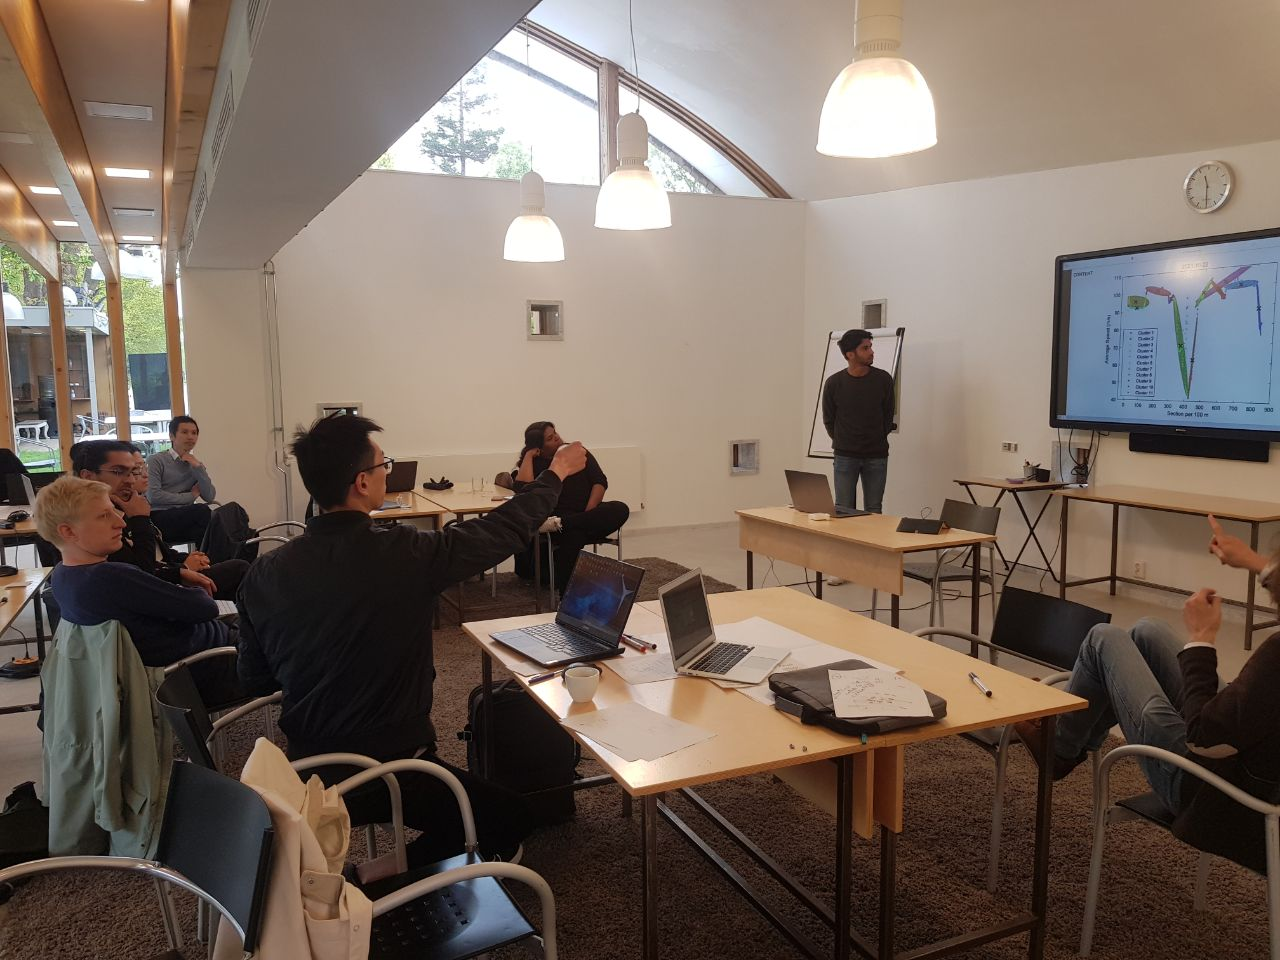
\includegraphics[width=3cm]{photo1.jpg}
    \caption{Caption}
    \label{fig:picture1}
\end{figure}

\begin{figure}
    \centering
    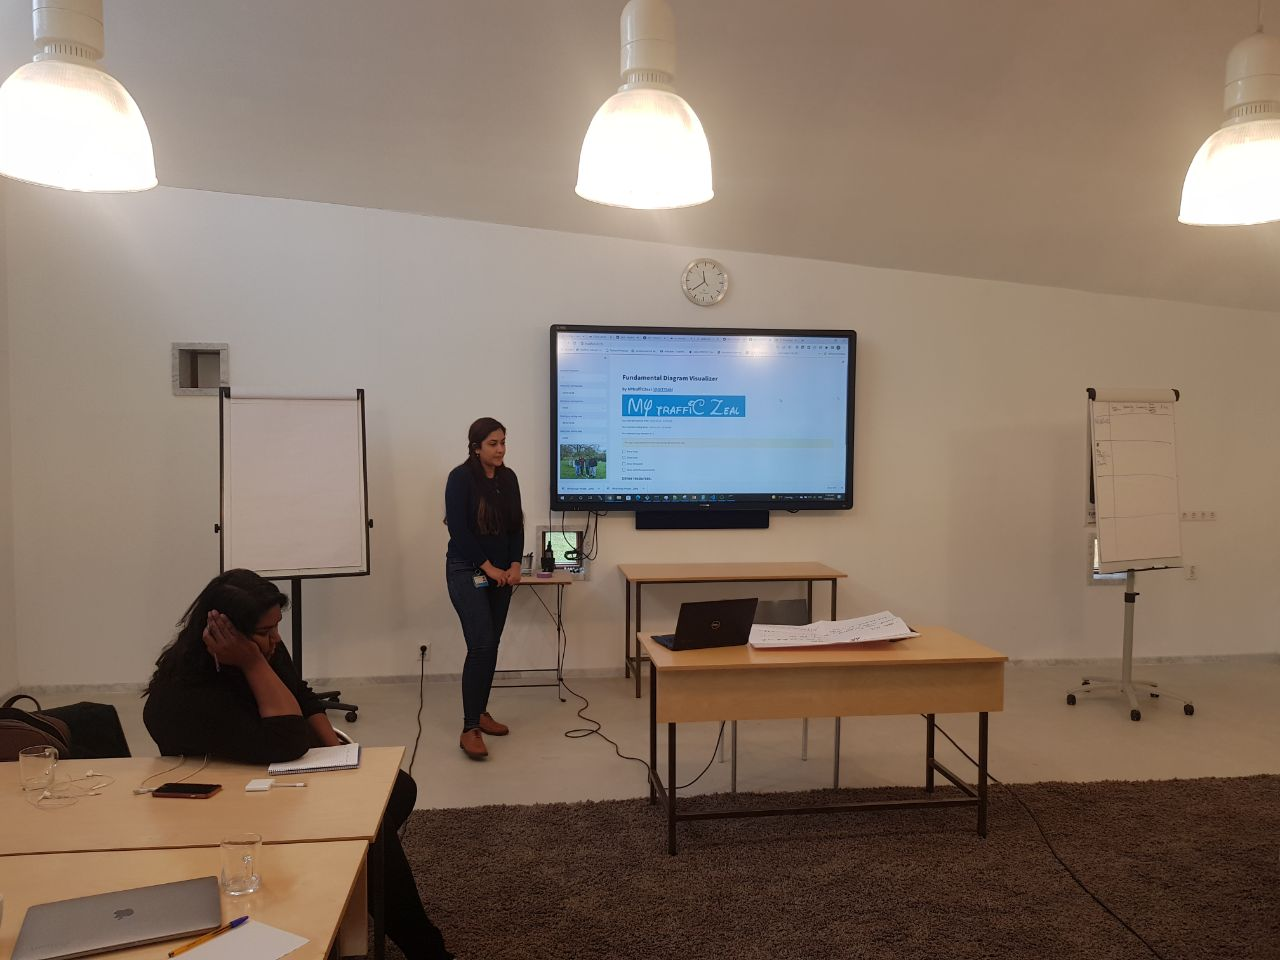
\includegraphics[width=3cm]{photo2.jpg}
    \caption{Caption}
    \label{fig:picture2}
\end{figure}

\subsection{Lists}

In this part we are going to make a few lists:
\begin{itemize}
    \item a bullet list (this one)
    \item the bullets can change 'globally' by redefined by
    
    \verb|\renewcommand{\labelitemi}{$\heartsuit$}|
    \item an enumeration
    \begin{itemize}
        \item[$+$] positive subitem
        \item[$-$] negative subitem
        \item[$\heartsuit$] heartsuit subitem
    \end{itemize}
\end{itemize}

This is an enumeration of the floating environments:
\begin{enumerate}
    \item figures
    \item table
\end{enumerate}

Another type of list is called a description:
\begin{description}
\item[rotating]
is a package that provides the couple of environments for including wide floats on one single, rotated page.
\item[longtable]
gives you the possibility to write long tables that are automatically split between pages.
\item[pdfscape]
provides an environment for rotating the pages sideways in a section of your document. Together with longtable it can be used to insert a table that is long as well as wide.
\end{description}

\subsection{Tables}

This section holds some examples of tables. Initially a basic table formatted using 'siunitx', then rotated wide table, and finally a multipage 'longtable'. Some tabular material to give you a head start can be found in \verb|https://novanext.nl/latex/trees|.

\begin{table}
    \centering
    \caption{Some optimistic number}
    \begin{tabular}{lcc}
        \toprule
                 & {Mass} & {Stiffness}  \\
                 
        \midrule
            First row   &   2.71828 &   \num{1.024e3} \\
            Second row  &   \num{31.4159} &   \num{63.151e3} \\
            Third row   &   \num{161.803398}  &   \num{12.5e-3}   \\
        \bottomrule
    \end{tabular}
    \label{tab:my_label}
\end{table}